\chapter{Introducción}
\label{cap:introduccion}

\chapterquote{People think of education as something that they can finish.}{Isaac Asimov}
\section{¿Qué es APRS?}

El APRS o Sistema Automático de Reporte de Paquetes (APRS, por sus siglas en inglés: Automatic Packet Reporting System) es un sistema de comunicaciones digitales en tiempo real que permite el intercambio de información entre estaciones de radioaficionados.

De manera general, APRS se utiliza para el rastreo de vehículos, la transmisión de mensajes de texto, la diseminación de información meteorológica y la comunicación en situaciones de emergencia aunque debido a la flexibilidad del protocolo puede ser usado en muchas otras situaciones.

\begin{figure}[h!]
	\centering
	
\includegraphics[width=0.25\textwidth]{Imagenes/Chapter_1/APRS_logo.png}
	\caption{Logo de APRS.}
	\label{fig:aprs-logo-es}
\end{figure}

\section{Características principales de APRS}

APRS posee varias características que lo hacen útil y versátil en el ámbito de la comunicación de radioaficionados, entre las cuales se encuentran las siguientes:
\begin{itemize}
	\item \textbf{Frecuencia de operación:} APRS opera en la banda de VHF, específicamente en la frecuencia de 144.80 MHz en Europa, aunque en otras regiones del mundo se utilizan frecuencias diferentes, tal como se muestra en la figura \Cref{fig:freq-map-es}.
	\item \textbf{Modo de transmisión:} APRS utiliza como modo de transmisión paquetes individuales que han de seguir un formato establecido, esto facilita enormemente la adopción e integración de esta tecnología.
	\item \textbf{Actualización de fatos en APRS:} En el sistema APRS, un paquete de información se transmite múltiples veces, disminuyendo gradualmente la frecuencia de envío de estas transmisiones a medida que el tiempo avanza. Este método tiene como objetivo maximizar la tasa de recepción de los paquetes.
\end{itemize}

\begin{figure}[h]
	\centering
	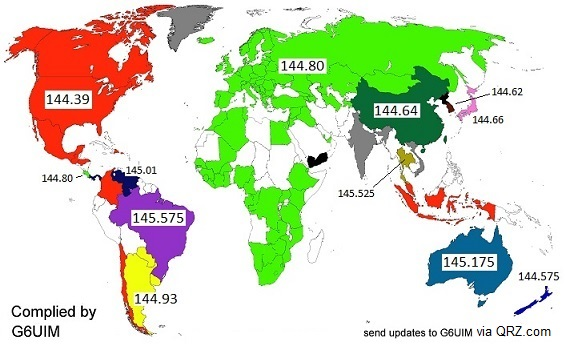
\includegraphics[width=0.65\textwidth]{Imagenes/Chapter_1/mapa_frecuencias_aprs.jpg}
	\caption{Mapa de frecuencias APRS en el mundo.}
	\label{fig:freq-map-es}
\end{figure}


\section{Usos principales de APRS}

\begin{itemize}
	\item \textbf{Reportes GPS:} APRS permite a los usuarios enviar su ubicación geográfica en forma de coordenadas, obtenida a través de sistemas GPS, lo que facilita el seguimiento de vehículos o personas en tiempo real.

	\item \textbf{Datos meteorológicos:} Las estaciones meteorológicas suelen utilizar mensajes APRS para reportar diferentes datos como temperatura, humedad o presión barométrica, incluyendo información actualizada y útil para diversas aplicaciones.

	\item \textbf{Integración con internet:} Mediante el sistema APRS-IS, los mensajes APRS son accesibles desde internet a través de distintos nodos, ampliando el alcance y la extensión de este sistema.

	\item \textbf{Uso en emergencias:} En situaciones de emergencia, APRS es una herramienta vital para la comunicación de \textit{broadcast} y el seguimiento de recursos y personal.
\end{itemize}

\section{Historia y desarrollo de APRS}

El sistema APRS nació en la década de los 80 de la mano de Bob Bruninga, un ingeniero que trabajaba en la Academia Naval de los Estados Unidos. Bruninga creó la primera implementación de APRS en un ordenador Apple II en 1982 con el objetivo de mapear informes de posición de la Marina en alta frecuencia. \cite{APRSOrigins}

El primer uso real del APRS fue en 1984, cuando Bruninga desarrolló una versión más avanzada en un VIC-20 para reportar la posición y el estado de los caballos de una carrera de resistencia.

Durante los siguientes años, Bruninga continuó perfeccionando el sistema, al que posteriormente bautizó como Sistema de Tráfico de Emergencia Sin Conexión (CETS, por sus siglas en inglés).

Tras una serie de ejercicios de la Agencia Federal de Gestión de Emergencias (FEMA) usando CETS, el sistema fue trasladado al IBM PC. Durante la década de los 90, CETS (ya conocido como el Sistema de Reporte Automático de Posición) continuó evolucionando.

A medida que la tecnología GPS se volvía más ampliamente disponible, el término ``Posición'' se reemplazó por ``Paquete'' para representar mejor las capacidades más generales del sistema y enfatizar sus usos más allá del mero reporte de posición.

\begin{figure}[h]
	\centering
	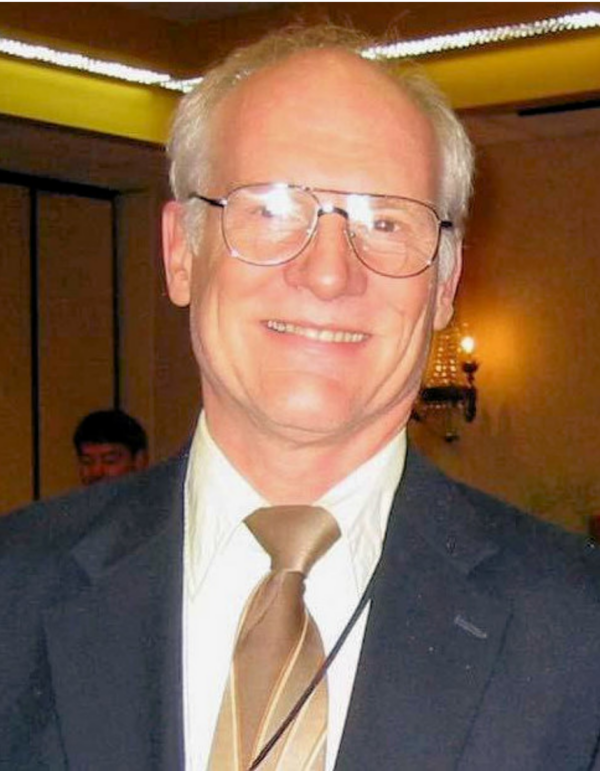
\includegraphics[width=0.2\textwidth]{Imagenes/Chapter_1/bob_bruninga.png}
	\caption{Bob Bruninga (creador del sistema APRS).}
	\label{fig:bob-bruninga-es}
\end{figure}


\section{Proposal and Objectives}

A comprehensive solution is proposed to encompass the acquisition, processing, visualization, and analysis of APRS data.

\subsection{Objectives}

The aim of the project is to develop a solution that enhances user experience and enriches available APRS information through the integration of data from various open and accessible sources.

\subsection{Enfoque}

\begin{itemize}
    \item \textbf{Experiencia de usuario mejorada:} La solución tendrá una interfaz intuitiva, rápida y útil que facilite la navegación y la interacción con los datos.
    
    \item \textbf{Análisis avanzado:} La solución contará con herramientas avanzadas para la visualización detallada del tráfico APRS, filtrado preciso y análisis de datos, con el objetivo de extraer inteligencia de los mensajes recibidos.
    
    \item \textbf{Complementación:} La solución no tiene como objetivo sustituir a aprs.fi, aprs.to u otras plataformas similares, sino ofrecer una alternativa con funcionalidades complementarias que enriquezcan la experiencia del usuario.
    
    \item \textbf{Enriquecimiento de información:} Se recopilarán datos provenientes de diversas fuentes abiertas y disponibles para ofrecer una visión más completa del tráfico APRS y sus usuarios, mejorando así la calidad de la información disponible para los usuarios.
\end{itemize}

\subsection{Beneficios}

\begin{itemize}
    \item \textbf{Mayor comprensión del tráfico APRS:} Los usuarios podrán obtener información más detallada y procesable a partir de los mensajes transmitidos, lo que les permitirá una mayor comprensión del tráfico APRS.
    
	\item \textbf{Toma de decisiones más efectiva:} El análisis de datos integrado ayudará a los usuarios a tomar decisiones más informadas haciendo uso de la información recibida, mejorando así la eficacia de sus acciones.
    
    \item \textbf{Flexibilidad:} La opción de auto-alojamiento permitirá a los usuarios tener un mayor control sobre sus datos y privacidad, proporcionando así una mayor flexibilidad en cuanto a su gestión.
\end{itemize}

\section{Requisitos}
\label{sec:Requisitos}

La solución propuesta debe cumplir con una serie de requisitos imprescindibles para asegurar su utilidad y accesibilidad:

\begin{itemize}
    \item \textbf{Bajo costo:} La solución debe ser económica para garantizar su accesibilidad a una amplia gama de usuarios, incluidos aquellos con presupuestos limitados.
    
    \item \textbf{Flexibilidad de alojamiento:} La solución debe ofrecer la capacidad de auto-alojamiento, los usuarios deben poder optar por alojarla en sus propios servidores o usar la solución en la nube según sus preferencias y requisitos específicos.
    
    \item \textbf{Extensible:} La solución debe ser extensible, lo que significa que debe permitir la integración de nuevas funcionalidades y la expansión de su capacidad según las necesidades cambiantes de los usuarios.
    
    \item \textbf{Mejor filtrado:} Se debe ofrecer un filtrado más preciso y flexible en comparación con las plataformas existentes, lo que permitirá a los usuarios obtener información relevante y útil de los datos APRS para complementar la ya provista por las alternativas.
    
	\item \textbf{Análisis de datos integrado:} La solución debe incluir un análisis de datos integrado para ayudar a los usuarios a comprender mejor la información recibida a través del APRS y obtener perspectivas y conclusiones valiosas a partir de los mensajes transmitidos.
	
\end{itemize}

\section{Plan de trabajo}

Para la realización de este proyecto se ha propuesto el siguiente plan de trabajo, que se divide en las siguientes fases:

\begin{itemize}
	\item \textbf{Fase 1:} Investigación y Análisis de Requisitos.
	\item \textbf{Fase 2:} Diseño y Planificación.
	\item \textbf{Fase 3:} Implementación y Desarrollo.
	\item \textbf{Fase 4:} Realización de la memoria.
\end{itemize}

\noindent En la figura \Cref{fig:gantt-diagram-es} se muestra el diagrama de Gantt con las fechas de inicio y fin de cada una de las actividades que se han llevado a cabo a lo largo del proyecto.

\begin{figure}[h]
	\centering
	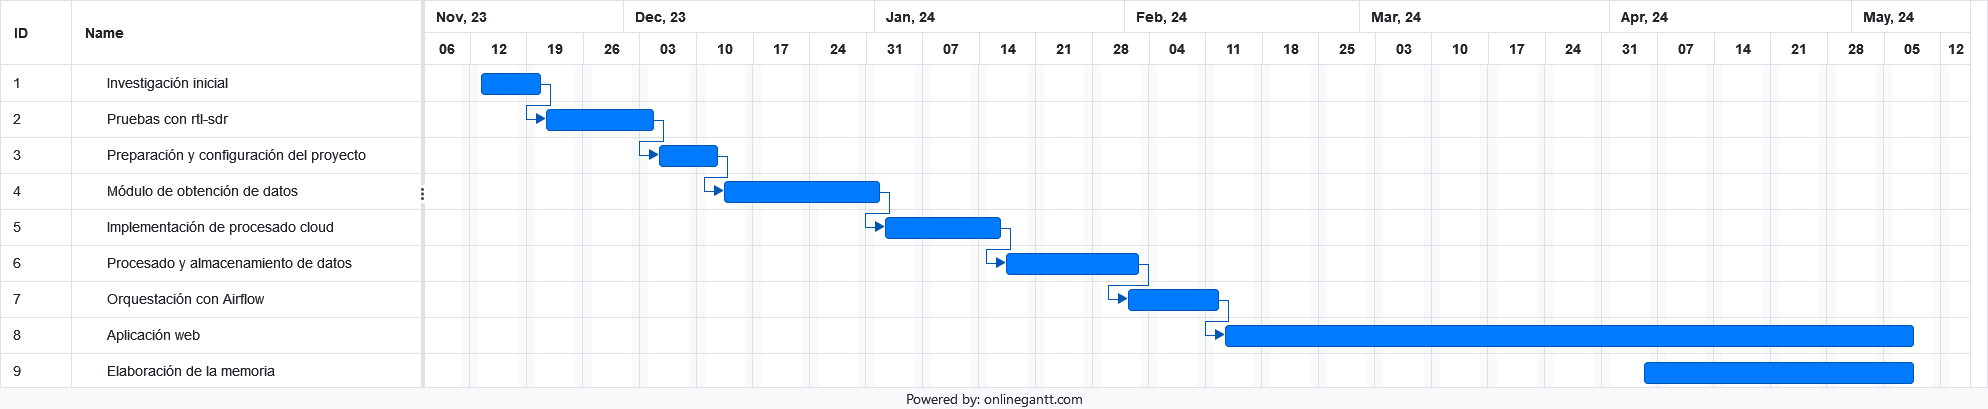
\includegraphics[width=1\textwidth]{Imagenes/Chapter_1/gant.png}
	\caption{Plan de trabajo propuesto.}
	\label{fig:gantt-diagram-es}
\end{figure}

\noindent También se han realizado reuniones periódicas con los directores de TFG para revisar el progreso y discutir los problemas encontrados durante el desarrollo.